%package list
\documentclass{article}
\usepackage[top=3cm, bottom=3cm, outer=3cm, inner=3cm]{geometry}
\usepackage{multicol}
\usepackage{graphicx}
\usepackage{url}
%\usepackage{cite}
\usepackage{hyperref}
\usepackage{array}
%\usepackage{multicol}
\newcolumntype{x}[1]{>{\centering\arraybackslash\hspace{0pt}}p{#1}}
\usepackage{natbib}
\usepackage{pdfpages}
\usepackage{multirow}
\usepackage[normalem]{ulem}
\useunder{\uline}{\ul}{}
\usepackage{svg}
\usepackage{xcolor}
\usepackage{listings}
\lstdefinestyle{ascii-tree}{
    literate={├}{|}1 {─}{--}1 {└}{+}1 
  }
\lstset{basicstyle=\ttfamily,
  showstringspaces=false,
  commentstyle=\color{red},
  keywordstyle=\color{blue}
}
\lstset{basicstyle=\ttfamily\fontfamily{Consolas}\selectfont,
	showstringspaces=false,
	commentstyle=\color{red},
	keywordstyle=\color{blue},
	literate={á}{{\'a}}1 {é}{{\'e}}1 {í}{{\'i}}1 {ó}{{\'o}}1 {ú}{{\'u}}1 {ñ}{{\~n}}1 {Á}{{\'A}}1 {É}{{\'E}}1 {Í}{{\'I}}1 {Ó}{{\'O}}1 {Ú}{{\'U}}1 {ñ}{{\~n}}1 {Ñ}{{\~N}}1 {ü}{{\"u}}1 {Ü}{{\"U}}1 {¡}{{!`}}1 {¿}{{?`}}1
}
%\usepackage{booktabs}
\usepackage{caption}
\usepackage{subcaption}
\usepackage{float}
\usepackage{array}

\newcolumntype{M}[1]{>{\centering\arraybackslash}m{#1}}
\newcolumntype{N}{@{}m{0pt}@{}}


%%%%%%%%%%%%%%%%%%%%%%%%%%%%%%%%%%%%%%%%%%%%%%%%%%%%%%%%%%%%%%%%%%%%%%%%%%%%
%%%%%%%%%%%%%%%%%%%%%%%%%%%%%%%%%%%%%%%%%%%%%%%%%%%%%%%%%%%%%%%%%%%%%%%%%%%%
\newcommand{\itemEmail}{jcondorios@unsa.edu.pe \par jcusilaymeg@unsa.edu.pe \par almamanima@unsa.edu.pe \par cvaldivialu@unsa.edu.pe}
\newcommand{\itemStudent}{Condorios Yllapuma Jorge \par Cusilayme García José Luis \par Mamani Mamani Alexis \par Valdivia Luna Carlo Joaquín}
\newcommand{\itemProffesor}{Mg. Edith Giovanna Cano Mamani}
\newcommand{\itemProffEmail}{ecanoma@unsa.edu.pe}
\newcommand{\itemCourse}{Estructura de Datos}
\newcommand{\itemCourseCode}{20222076 \par 20220598 \par 20222066  \par 20220567}
\newcommand{\itemSemester}{III}
\newcommand{\itemUniversity}{Universidad Nacional de San Agustín de Arequipa}
\newcommand{\itemFaculty}{Facultad de Ingeniería de Producción y Servicios}
\newcommand{\itemDepartment}{Departamento Académico de Ingeniería de Sistemas e Informática}
\newcommand{\itemSchool}{Escuela Profesional de Ingeniería de Sistemas}
\newcommand{\itemAcademic}{2023 - A}
\newcommand{\itemInput}{Del 16 Julio 2023}
\newcommand{\itemOutput}{Al 08 Agosto 2023}
\newcommand{\itemPracticeNumber}{Detector de Plagio}
\newcommand{\itemTheme}{Proyecto Final}
%%%%%%%%%%%%%%%%%%%%%%%%%%%%%%%%%%%%%%%%%%%%%%%%%%%%%%%%%%%%%%%%%%%%%%%%%%%%
%%%%%%%%%%%%%%%%%%%%%%%%%%%%%%%%%%%%%%%%%%%%%%%%%%%%%%%%%%%%%%%%%%%%%%%%%%%%

\usepackage[english,spanish]{babel}
\usepackage[utf8]{inputenc}
\AtBeginDocument{\selectlanguage{spanish}}
\renewcommand{\figurename}{Figura}
\renewcommand{\refname}{Referencias}
\renewcommand{\tablename}{Tabla} %esto no funciona cuando se usa babel
\AtBeginDocument{%
	\renewcommand\tablename{Tabla}
}

\usepackage{fancyhdr}
\pagestyle{fancy}
\fancyhf{}
\setlength{\headheight}{30pt}
\renewcommand{\headrulewidth}{1pt}
\renewcommand{\footrulewidth}{1pt}
\fancyhead[L]{\raisebox{-0.2\height}{
\includegraphics[width=3cm]{img/logo_episunsa.png}}}
\fancyhead[C]{\fontsize{7}{7}\selectfont	\itemUniversity \\ \itemFaculty \\ \itemDepartment \\ \itemSchool \\ \textbf{\itemCourse}}
\fancyhead[R]{\raisebox{-0.2\height}{
\includegraphics[width=1.2cm]{img/logo_abet}}}
\fancyfoot[L]{Grupo EDA}
\fancyfoot[C]{\itemCourse}
\fancyfoot[R]{Página \thepage}

% para el codigo fuente
\usepackage{listings}
\usepackage{color, colortbl}
\definecolor{dkgreen}{rgb}{0,0.6,0}
\definecolor{gray}{rgb}{0.5,0.5,0.5}
\definecolor{mauve}{rgb}{0.58,0,0.82}
\definecolor{codebackground}{rgb}{0.95, 0.95, 0.92}
\definecolor{tablebackground}{rgb}{0.8, 0, 0}

\lstset{frame=tb,
	language=bash,
	aboveskip=3mm,
	belowskip=3mm,
	showstringspaces=false,
	columns=flexible,
	basicstyle={\small\ttfamily},
	numbers=none,
	numberstyle=\tiny\color{gray},
	keywordstyle=\color{blue},
	commentstyle=\color{dkgreen},
	stringstyle=\color{mauve},
	breaklines=true,
	breakatwhitespace=true,
	tabsize=3,
	backgroundcolor= \color{codebackground},
}

\begin{document}
	
	\vspace*{10px}
	
	\begin{center}	
		\fontsize{17}{17} \textbf{ Informe de Laboratorio \itemPracticeNumber}
	\end{center}
	\centerline{\textbf{\Large Tema: \itemTheme}}
	%\vspace*{0.5cm}	

	\begin{flushright}
		\begin{tabular}{|M{2.5cm}|N|}
			\hline 
			\rowcolor{tablebackground}
			\color{white} \textbf{Nota}  \\
			\hline 
			     \\[30pt]
			\hline 			
		\end{tabular}
	\end{flushright}	

	\begin{table}[H]
		\begin{tabular}{|x{4.7cm}|x{4.8cm}|x{4.8cm}|}
			\hline 
			\rowcolor{tablebackground}
			\color{white} \textbf{Estudiante} & \color{white}\textbf{CUI}  & \color{white}\textbf{Correo} \\
			\hline 
			{\itemStudent} & {\itemCourseCode} & {\itemEmail }     \\
			\hline 			
		\end{tabular}
	\end{table}		
	
	\begin{table}[H]
		\begin{tabular}{|x{4.7cm}|x{4.8cm}|x{4.8cm}|}
			\hline 
			\rowcolor{tablebackground}
			\color{white} \textbf{Facultad} & \color{white}\textbf{Asignatura}  & \color{white}\textbf{Docente}\\
			\hline 
			{\itemSchool} & {\itemCourse \par Semestre: \itemSemester}   & {\itemProffesor \par \itemProffEmail} \\
			\hline 			
		\end{tabular}
	\end{table}	
	
	\begin{table}[H]
		\begin{tabular}{|x{4.7cm}|x{4.8cm}|x{4.8cm}|}
			\hline 
			\rowcolor{tablebackground}
			\color{white}\textbf{Laboratorio} & \color{white}\textbf{Tema}  & \color{white}\textbf{Duración}   \\
			\hline 
			\itemPracticeNumber & \itemTheme & 02 horas   \\
			\hline 
		\end{tabular}
	\end{table}
	
	\begin{table}[H]
		\begin{tabular}{|x{4.7cm}|x{4.8cm}|x{4.8cm}|}
			\hline 
			\rowcolor{tablebackground}
			\color{white}\textbf{Semestre académico} & \color{white}\textbf{Fecha de inicio}  & \color{white}\textbf{Fecha de entrega}   \\
			\hline 
			\itemAcademic & \itemInput &  \itemOutput  \\
			\hline 
		\end{tabular}
	\end{table}
	
	\section{Tarea}
	\begin{itemize}		
		\item Este proyecto tiene por objetivo que los alumnos implementen un sistema de detección de plagio simple (sistema a ser implementado), en el cual, usando como referencia una base de datos, el usuario del sistema enviará un párrafo escrito por el mismo (o copiado de alguna fuente) y lo enviará al sistema, el cual se encarga de realizar las consultas sobre la base de datos a fin de determinar si existió plagio o no.
		\item Consideraciones:
		\begin{itemize}
		\item  \textbf{Eficiencia del sistema:}  En general, los sistemas priman la eficiencia y la velocidad con la que realizan sus funcionalidades, y en este proyecto no podíamos dejar de lado esto.
		Garantizar velocidad en detectores de plagio muchas veces requiere que se realicen pre-procesamientos sobre los textos, a fin de reducir la cantidad de contenido a ser consultado.
		\item \textbf{Pre-procesamientos comunes incluyen:} eliminación de caracteres especiales (por ejemplo, puntos, comas, parentesis, etc.), extracción de raíces de las palabras (por ejemplo, “act-” sería la raíz de las palabras “actor”, “actores”, “actriz”, etc.), etc. Estos pre-procesamientos reducen considerablemente la complejidad de la búsqueda de coincidencias, pues son menos comparaciones a ser realizadas. 
		Sin embargo, el uso de pre-procesamientos algunas veces impactan en la eficiencia de la detección de plagio, pues se pierde la comparación exacta de palabras y
frases.
\item \textbf{Número de integrantes} Este proyecto será realizado en grupos entre 3 y 4 integrantes. Cada grupo tendrá un líder, el cual debe enviar en las fechas
correspondientes los diferentes entregables solicitados por los profesores.
		\end{itemize}
		
	\end{itemize}
		 
		
	\section{Equipos, materiales y temas utilizados}
	\begin{itemize}
		\item Sistema Operativo Windows 10 Home 64 bits (10.0, compilation 19045)
		\item VIM 9.0.
		\item OpenJDK 64-Bits 17.0.7.
		\item Git 2.39.2.
		\item Cuenta en GitHub con el correo institucional.
		\item Java 
	\end{itemize}
	
	\section{URL de Repositorio Github}
	\begin{itemize}
		\item URL del Repositorio GitHub para clonar o recuperar.
		\item \url{https://github.com/JorgeCY21/EDA_LAB_D}
		\item URL para el laboratorio 06 en el Repositorio GitHub.
		\item \url{https://github.com/JorgeCY21/EDA_LAB_D/tree/main/Lab_07}
	\end{itemize}
	
	\section{Actividades con el repositorio GitHub}
	
	\subsection{Creando e inicializando repositorio GitHub}
	\begin{itemize}
		\item Se realizaron los siguientes comandos en la computadora:
	\end{itemize}	
		
	\begin{lstlisting}[language=bash,caption={Dirijíéndonos al directorio de trabajo}][H]
		D:\
	\end{lstlisting}	
	\begin{lstlisting}[language=bash,caption={Clonando repositorio GitHub}][H]
		D:\ git clone https://github.com/JorgeCY21/EDA_LAB_D
	\end{lstlisting}
	\begin{lstlisting}[language=bash,caption={Inicializando directorio para laboratorio 06}][H]
		D:\ cd EDA_LAB_D
      D: \EDA_LAB_D> mkdir Lab_07
		D: \EDA_LAB_D> cd Lab_07
	\end{lstlisting}
	
	\subsection{Commits}
	\begin{lstlisting}[language=bash,caption={Commit: Creamos el trie principal}][H]
		
		D: \EDA_LAB_D\Lab_07> git add .
		D: \EDA_LAB_D\Lab_07> git commit -m ""	
		D: \EDA_LAB_D\Lab_07> git push -u origin main
	\end{lstlisting}
 	
	\section{Explicación de Código}
	 \subsection{Resumen}
	 \begin{minipage}{\textwidth}\setlength{\parskip}{2mm}
	 El proyecto \textbf{Detector de Plagio} es una aplicación de detección de plagio que utiliza estructuras Trie (árbol de prefijos) para almacenar y comparar palabras entre diferentes archivos y texto ingresado. 
	 
La aplicación permite a los usuarios cargar archivos de texto, ingresar texto manualmente y luego verificar si hay similitudes o plagio entre los contenidos de estos archivos y el texto ingresado, mostrando los resultados a través de una interfaz gráfica. La implementación incluye clases para la GUI, la gestión de resultados y la manipulación eficiente de estructuras Trie. 

El funcionamiento de este proyecto se divide en 4 componentes y se realiza de la siguiente manera:
\begin{itemize}
\item Los usuarios interactúan con la GUI para cargar archivos de texto, ingresar texto manualmente o realizar verificaciones de plagio. Mediante \textbf{GUI} (Clase): Se implementa la interfaz gráfica de usuario (GUI) 
\item La clase \textbf{PlagiarismChecker} maneja la carga de archivos y almacena su contenido en estructuras Trie. Proporciona métodos para verificar si un archivo contiene similitudes con otros archivos previamente cargados.
\item La clase \textbf{TrieNode} Implementa la estructura de nodo Trie, permitiendo la inserción y búsqueda eficiente de palabras, así como la comparación de contenido entre diferentes nodos Trie, normalizando las palabras para una comparación uniforme.
\item La clase \textbf{ResultChecker}Almacena y gestiona los resultados de detección de plagio para cada archivo, indicando si se encontraron similitudes o no.
\item Y finalmente la \textbf{GUI} muestra los resultados de detección de plagio a través de la interfaz, resaltando si se encontraron similitudes o no entre los contenidos.
\end{itemize}
	 \end{minipage}
	 \clearpage
	 \subsection{GUI}
	 \begin{itemize}
	 \item \textbf{Importación de paquetes:} Se importan diferentes clases y paquetes necesarios para construir la interfaz gráfica y realizar operaciones de lectura de archivos y detección de plagio.
	 \end{itemize}
	 \begin{figure}[H]
		\centering
		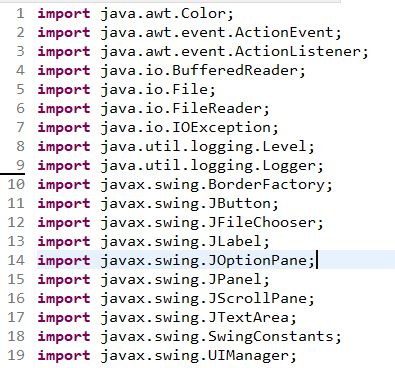
\includegraphics[width=0.8\textwidth,keepaspectratio]{img/GUI1.jpg}
		%\includesvg{img/automata.svg}
		%\label{img:mot2}
		%\caption{Product backlog.}
	\end{figure}
	
	\begin{itemize}
	\item \textbf{Variables de instancia y constantes:}
	 \begin{itemize}
	 \item \textbf{HEIGHT} y  \textbf{WIDTH}: Representan las dimensiones de la ventana.
	 \item\textbf{bodyPanel} Un panel donde se agregarán los componentes de la GUI.
	 \item Otros componentes como botones (btnVerifPlagio, btnSubirDoc, btnSubirArchivos), área de texto (textArea), seleccionador de archivos (fileChooser), entre otros.
	 \end{itemize}
	\end{itemize}
	 \begin{figure}[H]
		\centering
		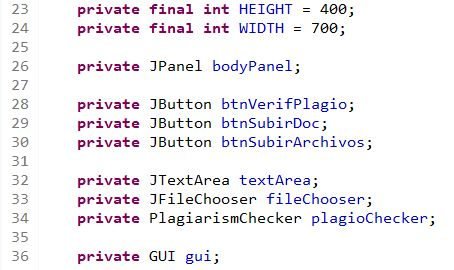
\includegraphics[width=0.8\textwidth,keepaspectratio]{img/GUI2.jpg}
		%\includesvg{img/automata.svg}
		%\label{img:mot2}
		%\caption{Product backlog.}
	\end{figure}
	
	\begin{itemize}
	\item \textbf{Constructor GUI:}
	 \begin{itemize}
	 \item Configura la apariencia y comportamiento de la ventana principal.
	 \item Inicializa \textbf{bodyPanel} y lo establece como el contenido de la ventana.
	 \item Llama a \textbf{initComponents()} para inicializar los componentes de la GUI.
	 \item Finalmente, se hace visible la ventana
	 \end{itemize}
	\end{itemize}
	 \begin{figure}[H]
		\centering
		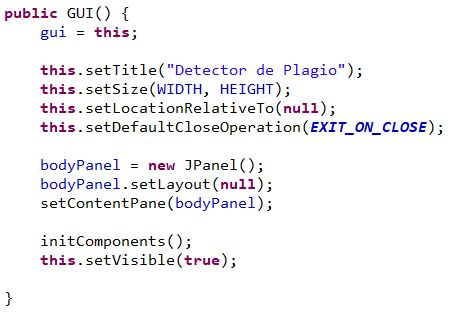
\includegraphics[width=0.8\textwidth,keepaspectratio]{img/GUI3.jpg}
		%\includesvg{img/automata.svg}
		%\label{img:mot2}
		%\caption{Product backlog.}
	\end{figure}
	
	\begin{itemize}
\clearpage	
	
	\item \textbf{Método initComponents():}
	 \begin{itemize}
	 \item Crea y coloca los componentes en el bodyPanel, como etiquetas, botones y un área de texto.
	 \item Asigna oyentes de eventos a los botones para manejar acciones como verificar plagio, cargar archivo y cargar archivos múltiples.
	 \end{itemize}
	\end{itemize}
	 \begin{figure}[H]
		\centering
		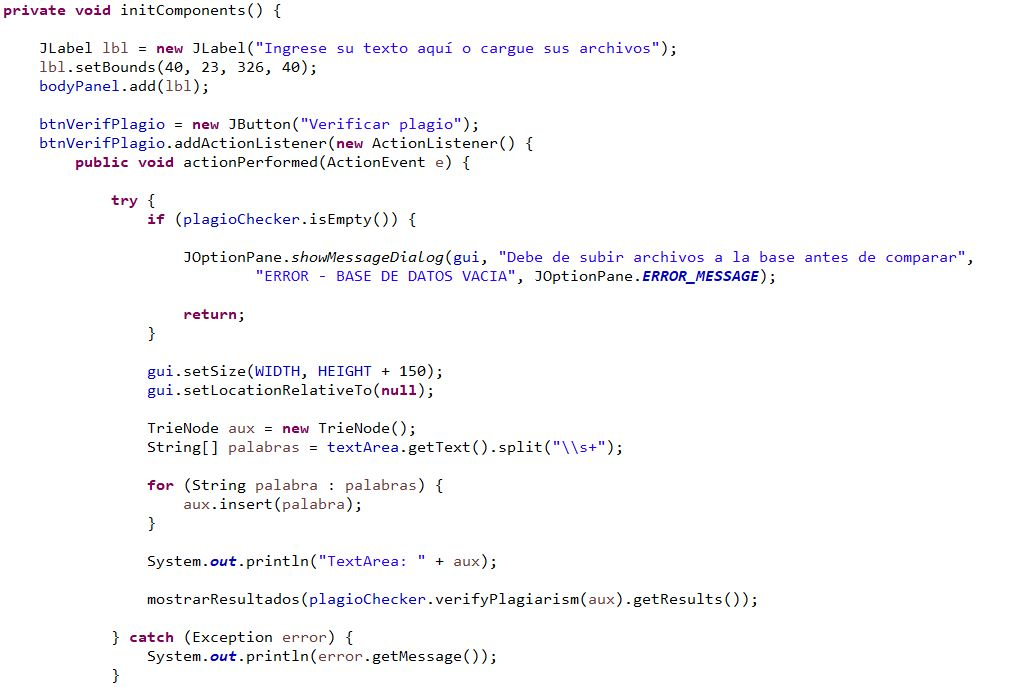
\includegraphics[width=0.8\textwidth,keepaspectratio]{img/GUI4.1.jpg}
		%\includesvg{img/automata.svg}
		%\label{img:mot2}
		%\caption{Product backlog.}
	\end{figure}
	\begin{figure}[H]
		\centering
		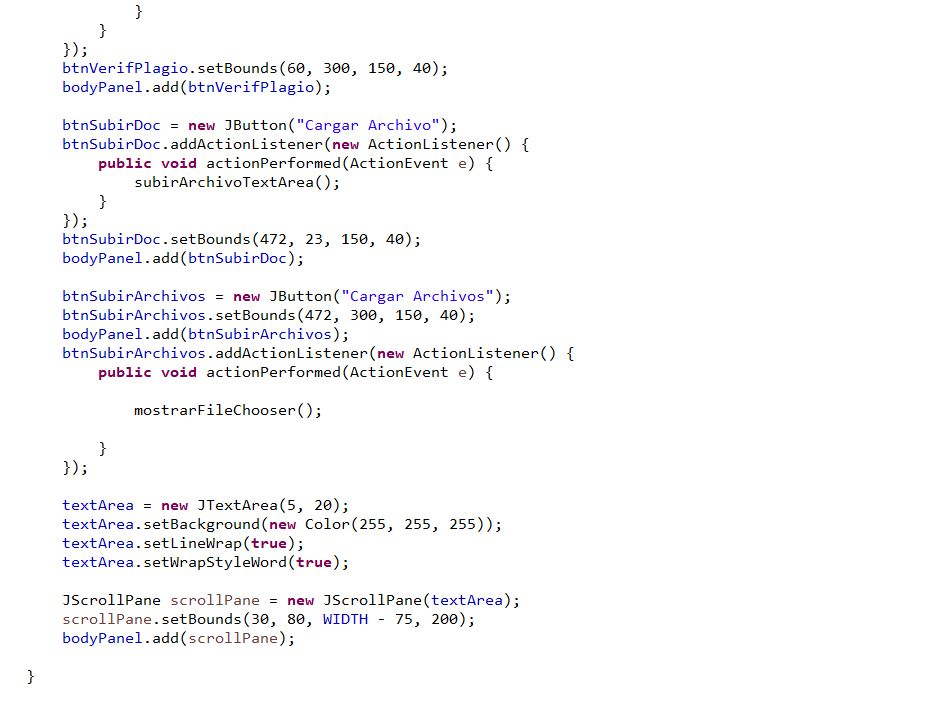
\includegraphics[width=0.8\textwidth,keepaspectratio]{img/GUI4.2.jpg}
		%\includesvg{img/automata.svg}
		%\label{img:mot2}
		%\caption{Product backlog.}
	\end{figure}
	
	\begin{itemize}
	\item \textbf{Método mostrarResultados(boolean[] results):}
	 \begin{itemize}
	 \item Recibe un arreglo de booleanos que representan los resultados de detección de plagio para diferentes archivos.
	 \item Crea y muestra etiquetas que indican si hubo plagio o no para cada archivo en la parte inferior de la ventana.
	 \end{itemize}
	\end{itemize}
	 \begin{figure}[H]
		\centering
		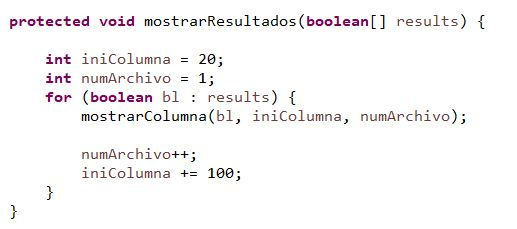
\includegraphics[width=0.8\textwidth,keepaspectratio]{img/GUI5.jpg}
		%\includesvg{img/automata.svg}
		%\label{img:mot2}
		%\caption{Product backlog.}
	\end{figure}
	
	\begin{itemize}
	\item \textbf{Método mostrarColumna(boolean bl, int iniColumna, int numArchivo):}
	 \begin{itemize}
	 \item Crea y coloca etiquetas y paneles de color para mostrar los resultados de plagio para cada archivo.
	 \end{itemize}
	\end{itemize}
	 \begin{figure}[H]
		\centering
		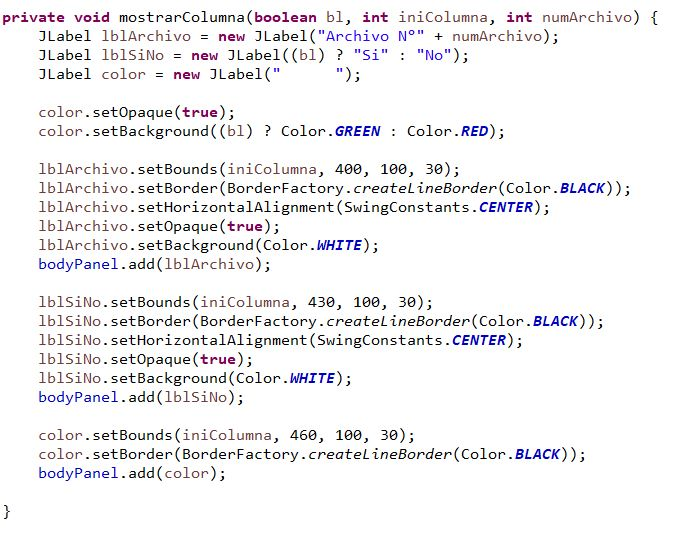
\includegraphics[width=0.8\textwidth,keepaspectratio]{img/GUI6.jpg}
		%\includesvg{img/automata.svg}
		%\label{img:mot2}
		%\caption{Product backlog.}
	\end{figure}
\clearpage		
	
	\begin{itemize}
	\item \textbf{Método subirArchivoTextArea():}
	 \begin{itemize}
	 \item Muestra un cuadro de diálogo para seleccionar un archivo.
	 \item Lee el contenido del archivo seleccionado y lo muestra en el área de texto.
	 \end{itemize}
	\end{itemize}
	 \begin{figure}[H]
		\centering
		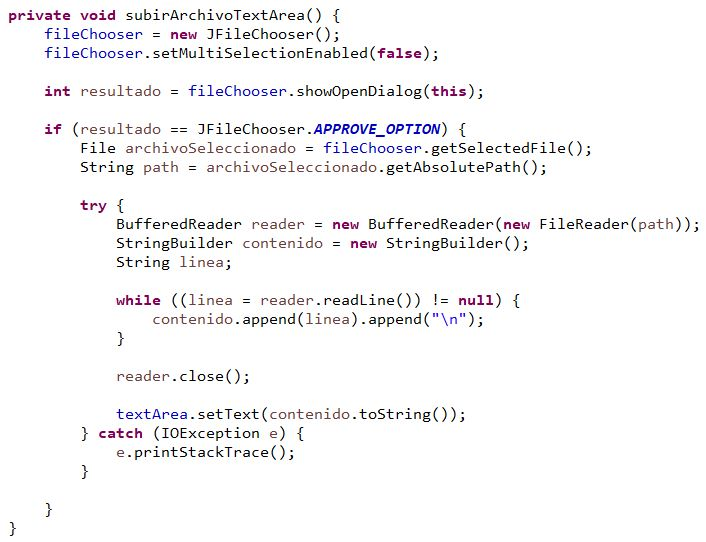
\includegraphics[width=0.8\textwidth,keepaspectratio]{img/GUI7.jpg}
		%\includesvg{img/automata.svg}
		%\label{img:mot2}
		%\caption{Product backlog.}
	\end{figure}
	
	\begin{itemize}
	\item \textbf{Método mostrarFileChooser():}
	 \begin{itemize}
	 \item Muestra un cuadro de diálogo para seleccionar múltiples archivos.
	 \item Inicializa un objeto PlagiarismChecker y carga los archivos seleccionados en él.
	 \end{itemize}
	\end{itemize}
	 \begin{figure}[H]
		\centering
		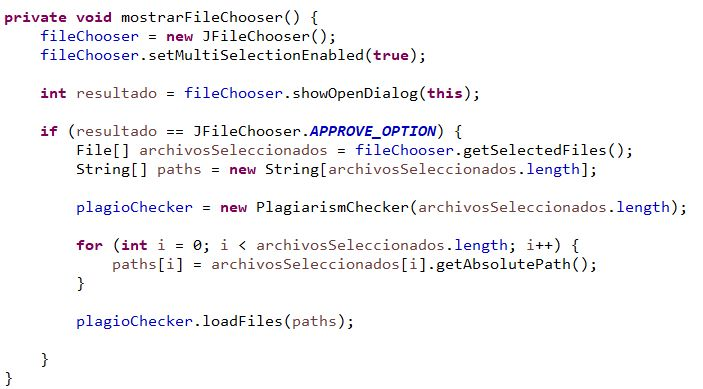
\includegraphics[width=0.8\textwidth,keepaspectratio]{img/GUI8.jpg}
		%\includesvg{img/automata.svg}
		%\label{img:mot2}
		%\caption{Product backlog.}
	\end{figure}
	
	\begin{itemize}
	\item \textbf{Método main(String args[]):}
	 \begin{itemize}
	 \item Llama al método mejorandoApariencia() para establecer la apariencia de la GUI.
	 \item Crea una instancia de la clase GUI, lo que inicia la aplicación.
	 \end{itemize}
	\end{itemize}
	 \begin{figure}[H]
		\centering
		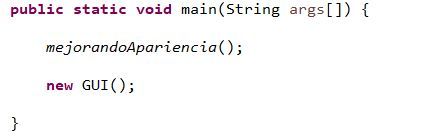
\includegraphics[width=0.8\textwidth,keepaspectratio]{img/GUI9.jpg}
		%\includesvg{img/automata.svg}
		%\label{img:mot2}
		%\caption{Product backlog.}
	\end{figure}
	
	\begin{itemize}
	\item \textbf{Método mejorandoApariencia():}
	 \begin{itemize}
	 \item Configura la apariencia de la GUI utilizando el LookAndFeel "Nimbus" para mejorar la presentación visual.
	 \end{itemize}
	\end{itemize}
	 \begin{figure}[H]
		\centering
		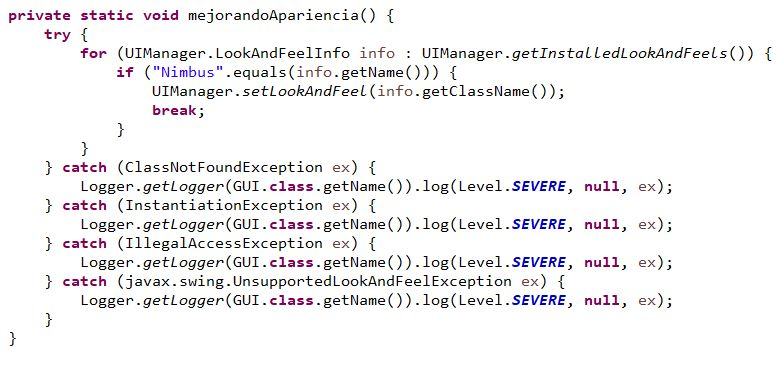
\includegraphics[width=0.8\textwidth,keepaspectratio]{img/GUI10.jpg}
		%\includesvg{img/automata.svg}
		%\label{img:mot2}
		%\caption{Product backlog.}
	\end{figure}
\clearpage	
	
	 \subsection{PlagiarismChecker}
	 \begin{itemize}
	\item \textbf{Definición de la clase PlagiarismChecker:} Esta clase parece ser parte del sistema de detección de plagio y está encargada de cargar y verificar la similitud entre archivos utilizando un enfoque basado en Trie (árbol de prefijos).
	\end{itemize}
	
	\begin{itemize}
	\item \textbf{Variables de instancia y constructor:}
	 \begin{itemize}
	 \item \textbf{Tries:} Un arreglo de nodos Trie (árbol de prefijos), uno para cada archivo a ser verificado.
	 \item \textbf{resultChecker:} Un objeto que parece ser responsable de verificar los resultados de plagio.
	 \item El constructor recibe la cantidad de archivos que se van a verificar y crea un arreglo de nodos Trie y un objeto ResultChecker.
	 \end{itemize}
	\end{itemize}
	 \begin{figure}[H]
		\centering
		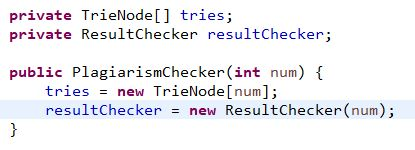
\includegraphics[width=0.8\textwidth,keepaspectratio]{img/PC1.jpg}
		%\includesvg{img/automata.svg}
		%\label{img:mot2}
		%\caption{Product backlog.}
	\end{figure}
	
	\begin{itemize}
	\item \textbf{Método loadFiles(String[] paths):}
	 \begin{itemize}
	 \item Carga los contenidos de los archivos especificados en los caminos de archivo dados en los nodos Trie correspondientes.
	 \item Devuelve \textbf{false} en este caso. No se manejan errores de lectura de archivos, solo se asume que todo funciona correctamente.
	 \end{itemize}
	\end{itemize}
	 \begin{figure}[H]
		\centering
		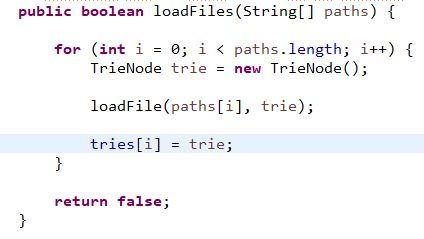
\includegraphics[width=0.8\textwidth,keepaspectratio]{img/PC2.jpg}
		%\includesvg{img/automata.svg}
		%\label{img:mot2}
		%\caption{Product backlog.}
	\end{figure}
\clearpage		
	
	\begin{itemize}
	\item \textbf{Método isEmpty():}
	 \begin{itemize}
	 \item Verifica si alguno de los nodos Trie está vacío (no se ha cargado ningún archivo).
	 \item Si al menos uno está vacío, devuelve true, lo que indica que la base de datos está vacía.
	 \end{itemize}
	\end{itemize}
	 \begin{figure}[H]
		\centering
		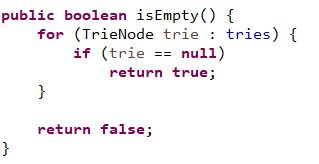
\includegraphics[width=0.8\textwidth,keepaspectratio]{img/PC3.jpg}
		%\includesvg{img/automata.svg}
		%\label{img:mot2}
		%\caption{Product backlog.}
	\end{figure}
	
	\begin{itemize}
	\item \textbf{Método loadFile(String path, TrieNode trie):}
	 \begin{itemize}
	 \item Lee el contenido del archivo especificado por \textbf{path}.
	 \item Divide cada línea en palabras y las inserta en el Trie especificado.
	 \item Devuelve \textbf{true} si la carga se realiza correctamente, y false si hay algún problema de lectura.
	 \end{itemize}
	\end{itemize}
	 \begin{figure}[H]
		\centering
		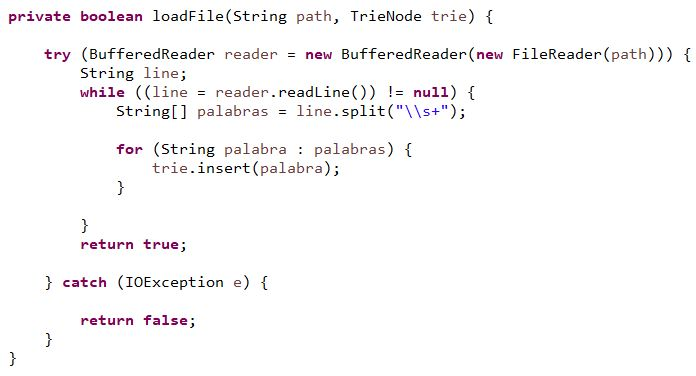
\includegraphics[width=0.8\textwidth,keepaspectratio]{img/PC4.jpg}
		%\includesvg{img/automata.svg}
		%\label{img:mot2}
		%\caption{Product backlog.}
	\end{figure}
\clearpage		
	
	\begin{itemize}
	\item \textbf{Método verifyPlagiarism(String path):}
	 \begin{itemize}
	 \item Este método parece estar incompleto, ya que solo retorna null. Parece que se supone que verificará la similitud de un archivo específico con respecto a los archivos ya cargados.
	 \end{itemize}
	\end{itemize}
	 \begin{figure}[H]
		\centering
		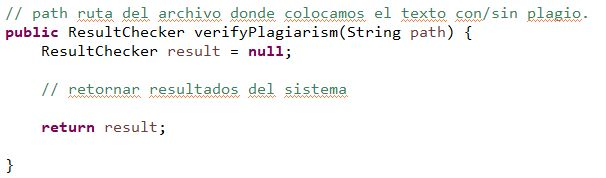
\includegraphics[width=0.8\textwidth,keepaspectratio]{img/PC5.jpg}
		%\includesvg{img/automata.svg}
		%\label{img:mot2}
		%\caption{Product backlog.}
	\end{figure}
	
	\begin{itemize}
	\item \textbf{Método verifyPlagiarism(TrieNode trie):}
	 \begin{itemize}
	 \item Recibe un nodo Trie que contiene las palabras del texto que se desea verificar.
	 \item Compara el nodo Trie recibido con cada uno de los nodos Trie almacenados en el arreglo \textbf{tries}.
	 \item Muestra información sobre los nodos Trie y establece si hay plagio o no en el objeto\textbf{resultChecker}.
	 \end{itemize}
	\end{itemize}
	 \begin{figure}[H]
		\centering
		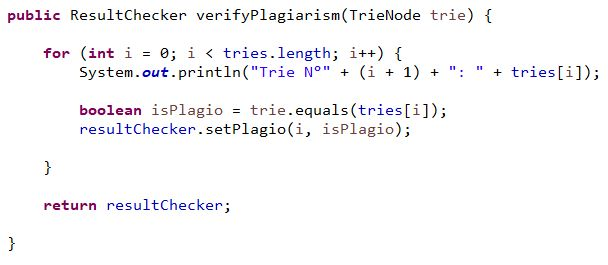
\includegraphics[width=0.8\textwidth,keepaspectratio]{img/PC6.jpg}
		%\includesvg{img/automata.svg}
		%\label{img:mot2}
		%\caption{Product backlog.}
	\end{figure}
	
	 \subsection{TrieNode}
	 \begin{itemize}
	\item \textbf{Definición de la clase TrieNode:} Esta clase implementa un nodo de un Trie (árbol de prefijos) para el almacenamiento y búsqueda eficiente de palabras en un contexto de detección de plagio.
	\end{itemize}
	
	\begin{itemize}
	\item \textbf{Variables de instancia y constructor:}
	 \begin{itemize}
	 \item \textbf{children:} Un mapa que asocia caracteres a nodos Trie hijos.
	 \item \textbf{isEndWord:} Un booleano que indica si el nodo Trie representa el final de una palabra.
	 \item El constructor inicializa el mapa de hijos y establece \textbf{isEndWord} en falso.
	 \end{itemize}
	\end{itemize}
	 \begin{figure}[H]
		\centering
		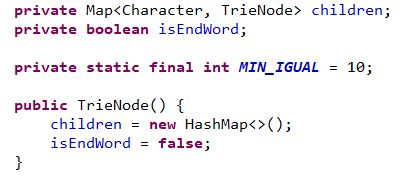
\includegraphics[width=0.8\textwidth,keepaspectratio]{img/TN1.jpg}
		%\includesvg{img/automata.svg}
		%\label{img:mot2}
		%\caption{Product backlog.}
	\end{figure}
	
	\begin{itemize}
	\item \textbf{Método insert(String word):}
	 \begin{itemize}
	 \item Inserta una palabra en el Trie, siguiendo el camino correspondiente en función de los caracteres de la palabra.
	 \item Normaliza la palabra usando el método normalizeWord() y luego itera sobre cada carácter para construir el Trie.
	 \end{itemize}
	\end{itemize}
	 \begin{figure}[H]
		\centering
		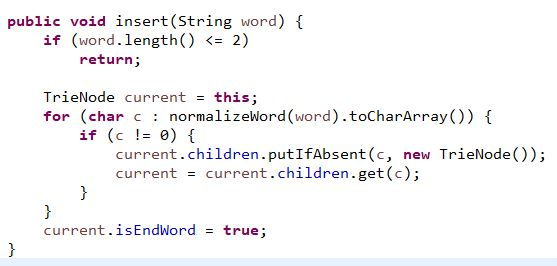
\includegraphics[width=0.8\textwidth,keepaspectratio]{img/TN2.jpg}
		%\includesvg{img/automata.svg}
		%\label{img:mot2}
		%\caption{Product backlog.}
	\end{figure}
	
	\begin{itemize}
	\item \textbf{Método search(String word):}
	 \begin{itemize}
	 \item Busca una palabra en el Trie, devolviendo verdadero si la palabra se encuentra en el Trie y representa el final de una palabra.
	 \end{itemize}
	\end{itemize}
	 \begin{figure}[H]
		\centering
		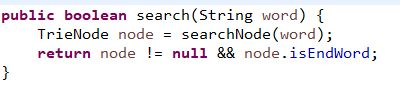
\includegraphics[width=0.8\textwidth,keepaspectratio]{img/TN3.jpg}
		%\includesvg{img/automata.svg}
		%\label{img:mot2}
		%\caption{Product backlog.}
	\end{figure}
	\clearpage
	
	\begin{itemize}
	\item \textbf{Método searchNode(String word):}
	 \begin{itemize}
	 \item Similar al método search(), pero devuelve el nodo Trie que representa el final de la palabra buscada en lugar de un booleano.
	 \end{itemize}
	\end{itemize}
	 \begin{figure}[H]
		\centering
		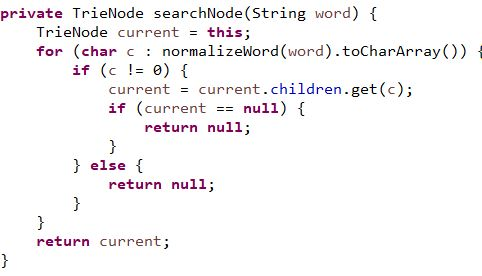
\includegraphics[width=0.8\textwidth,keepaspectratio]{img/TN4.jpg}
		%\includesvg{img/automata.svg}
		%\label{img:mot2}
		%\caption{Product backlog.}
	\end{figure}	
	
	\begin{itemize}
	\item \textbf{Método normalizeWord(String word):}
	 \begin{itemize}
	 \item Normaliza una palabra eliminando acentos y caracteres especiales, dejando solo letras minúsculas y números.
	 \end{itemize}
	\end{itemize}
	 \begin{figure}[H]
		\centering
		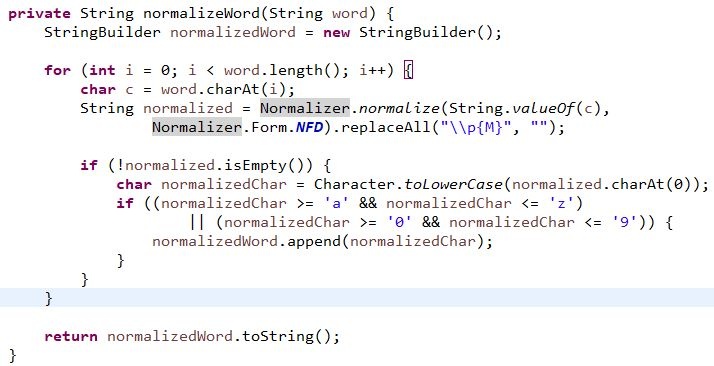
\includegraphics[width=0.8\textwidth,keepaspectratio]{img/TN5.jpg}
		%\includesvg{img/automata.svg}
		%\label{img:mot2}
		%\caption{Product backlog.}
	\end{figure}
	\clearpage
	
	\begin{itemize}
	\item \textbf{Método toString():}
	 \begin{itemize}
	 \item Devuelve una representación en cadena de todas las palabras almacenadas en el Trie.
	 \end{itemize}
	\end{itemize}
	 \begin{figure}[H]
		\centering
		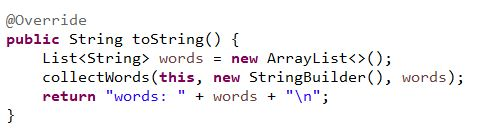
\includegraphics[width=0.8\textwidth,keepaspectratio]{img/TN6.jpg}
		%\includesvg{img/automata.svg}
		%\label{img:mot2}
		%\caption{Product backlog.}
	\end{figure}
	
	\begin{itemize}
	\item \textbf{Método equals(TrieNode datos):}
	 \begin{itemize}
	 \item Compara el contenido del Trie actual con otro Trie (datos) para determinar si hay una cantidad mínima de palabras en común, que se establece como MIN\_ IGUAL.
	 \end{itemize}
	\end{itemize}
	 \begin{figure}[H]
		\centering
		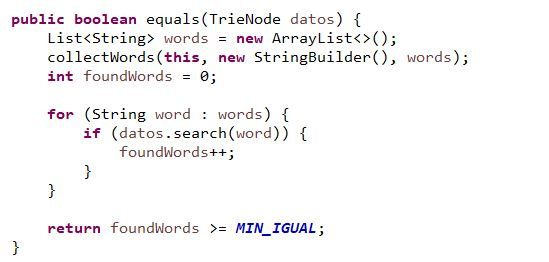
\includegraphics[width=0.8\textwidth,keepaspectratio]{img/TN7.jpg}
		%\includesvg{img/automata.svg}
		%\label{img:mot2}
		%\caption{Product backlog.}
	\end{figure}
	\clearpage
	
	\begin{itemize}
	\item \textbf{Método collectWords():}
	 \begin{itemize}
	 \item Recopila todas las palabras almacenadas en el Trie actual y las agrega a la lista \textbf{words}. 
	 \item Utiliza una técnica de búsqueda recursiva para explorar todas las combinaciones de letras.
	 \end{itemize}
	\end{itemize}
	 \begin{figure}[H]
		\centering
		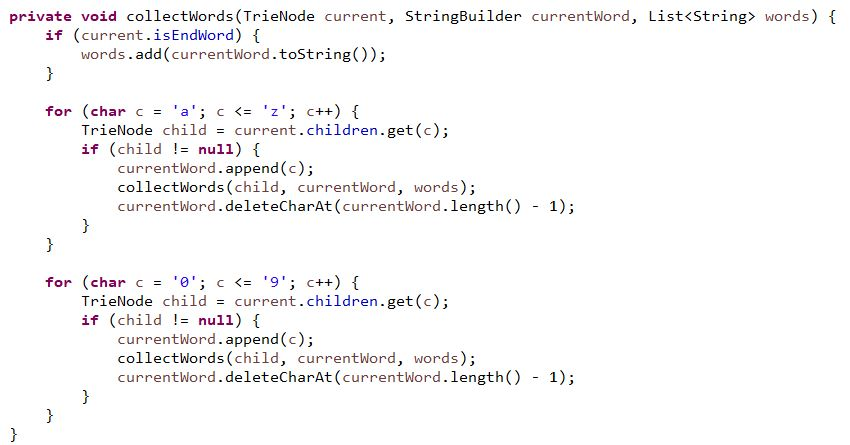
\includegraphics[width=1\textwidth,keepaspectratio]{img/TN8.jpg}
		%\includesvg{img/automata.svg}
		%\label{img:mot2}
		%\caption{Product backlog.}
	\end{figure}
	
	 \subsection{ResultChecker}
	\begin{itemize}
	\item \textbf{Definición de la clase ResultChecker:} Esta clase parece ser responsable de almacenar y gestionar los resultados de detección de plagio para cada archivo. Contiene métodos para configurar los resultados y obtenerlos.
	\end{itemize}	 
	
	\begin{itemize}
	\item \textbf{Método collectWords():}
	 \begin{itemize}
	 \item Recopila todas las palabras almacenadas en el Trie actual y las agrega a la lista \textbf{words}. 
	 \item Utiliza una técnica de búsqueda recursiva para explorar todas las combinaciones de letras.
	 \end{itemize}
	\end{itemize}
	
	\begin{itemize}
	\item \textbf{Método collectWords():}
	 \begin{itemize}
	 \item Recopila todas las palabras almacenadas en el Trie actual y las agrega a la lista \textbf{words}. 
	 \item Utiliza una técnica de búsqueda recursiva para explorar todas las combinaciones de letras.
	 \end{itemize}
	\end{itemize}
	
	\begin{itemize}
	\item \textbf{Variables de instancia y constructor:}
	 \begin{itemize}
	 \item \textbf{result:} Un arreglo de booleanos que almacena los resultados de detección de plagio para cada archivo. 
	 \item El constructor recibe la cantidad de archivos que se van a verificar y crea un arreglo de booleanos para almacenar los resultados.
	 \end{itemize}
	\end{itemize}
	
	\begin{itemize}
	\item \textbf{Método setPlagio(int index, boolean isPlagio):}
	 \begin{itemize}
	 \item Establece el resultado de detección de plagio para un archivo específico en el índice dado.
	 \item Recibe el índice del archivo y un valor booleano isPlagio que indica si se detectó plagio o no en ese archivo.
	 \item Actualiza el valor en el arreglo \textbf{result} en la posición correspondiente.
	 \end{itemize}
	\end{itemize}
	
	\begin{itemize}
	\item \textbf{Método getResults():}
	 \begin{itemize}
	 \item Devuelve el arreglo de booleanos result que contiene los resultados de detección de plagio para todos los archivos.
	 \end{itemize}
	\end{itemize}
	 \begin{figure}[H]
		\centering
		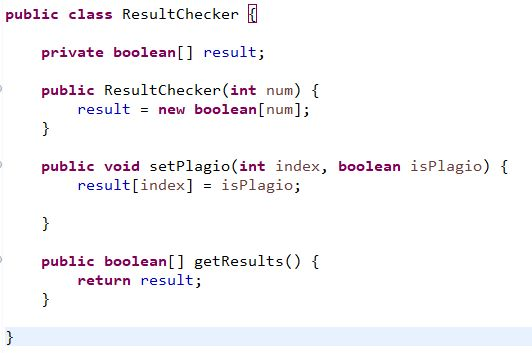
\includegraphics[width=1\textwidth,keepaspectratio]{img/RC.jpg}
		%\includesvg{img/automata.svg}
		%\label{img:mot2}
		%\caption{Product backlog.}
	\end{figure}
	 
 	
	\section{Códigos Fuente}	
	\lstinputlisting[language=Java, caption={GUI.java},numbers=left,]{src/GUI.java}
	
	\lstinputlisting[language=Java, caption={PlagiarismChecker.java},numbers=left,]{src/PlagiarismChecker.java}
	
	\lstinputlisting[language=Java, caption={ResultChecker.java},numbers=left,]{src/ResultChecker.java}
	 
	\lstinputlisting[language=Java, caption={TrieNode.java},numbers=left,]{src/TrieNode.java}
	
	\section{Ejecución Y pruebas}
	\begin{lstlisting}[language=bash,caption={Texto original a comparar}][H]
La inteligencia artificial es un campo de la informatica que se centra en la creacion de sistemas capaces de realizar tareas que normalmente requieren inteligencia humana. El cambio climatico es un fenomeno global que esta siendo causado en gran medida por la actividad humana, como la emision de gases de efecto invernadero.
	\end{lstlisting}
	\begin{lstlisting}[language=bash,caption={Texto con plagio 1}][H]
	La inteligencia artificial es un campo de la informatica que se centra en la creacion de sistemas capaces de realizar tareas que normalmente requieren inteligencia humana.
	\end{lstlisting}
	\begin{lstlisting}[language=bash,caption={Texto original sin plagio}][H]
	La robotica es una rama de la tecnologia que se ocupa del disenho, construccion y operacion de robots con el objetivo de automatizar y facilitar diversas tareas.
	\end{lstlisting}
	\begin{lstlisting}[language=bash,caption={Texto con plagio 2}][H]
	El cambio climatico es un fenomeno global que esta siendo causado en gran medida por la actividad humana, como la emision de gases de efecto invernadero.
	\end{lstlisting}
	\begin{figure}[H]
		\centering
		\caption{Ejecutamos el GUI}
		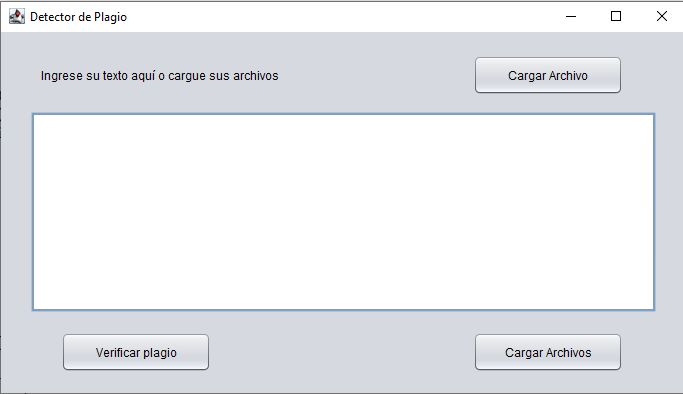
\includegraphics[width=1\textwidth,keepaspectratio]{img/Ejec1.jpg}
		%\includesvg{img/automata.svg}
		%\label{img:mot2}
		%\caption{Product backlog.}
	\end{figure}
	\begin{figure}[H]
		\centering
		\caption{Subimos el archivo original}
		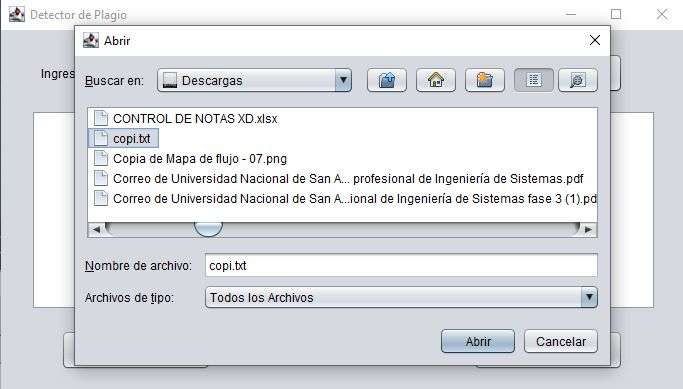
\includegraphics[width=1\textwidth,keepaspectratio]{img/Ejec2.jpg}
		%\includesvg{img/automata.svg}
		%\label{img:mot2}
		%\caption{Product backlog.}
	\end{figure}
	\begin{figure}[H]
		\centering
		\caption{Impresion del texto en el input de texto}
		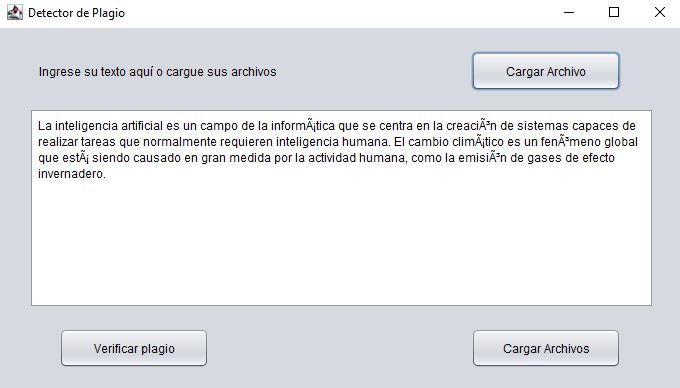
\includegraphics[width=1\textwidth,keepaspectratio]{img/Ejec3.jpg}
		%\includesvg{img/automata.svg}
		%\label{img:mot2}
		%\caption{Product backlog.}
	\end{figure}
	\begin{figure}[H]
		\centering
		\caption{Subimos los archivos que queremos comparar}
		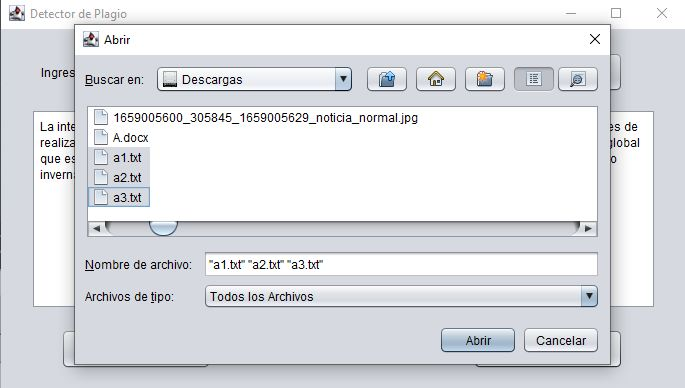
\includegraphics[width=1\textwidth,keepaspectratio]{img/Ejec4.jpg}
		%\includesvg{img/automata.svg}
		%\label{img:mot2}
		%\caption{Product backlog.}
	\end{figure}
	\begin{figure}[H]
		\centering
		\caption{Ejecucion Completa}
		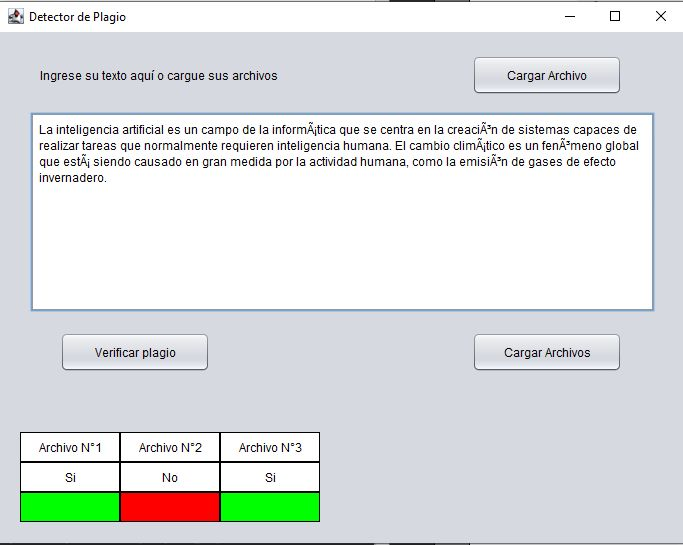
\includegraphics[width=1\textwidth,keepaspectratio]{img/EjecucionCompleta.jpg}
		%\includesvg{img/automata.svg}
		%\label{img:mot2}
		%\caption{Product backlog.}
	\end{figure}
		
	\section{\textcolor{red}{Rúbricas}}
	
	\subsection{\textcolor{red}{Entregable Informe}}
	\begin{table}[H]
		\caption{Tipo de Informe}
		\setlength{\tabcolsep}{0.5em} % for the horizontal padding
		{\renewcommand{\arraystretch}{1.5}% for the vertical padding
		\begin{tabular}{|p{3cm}|p{12cm}|}
			\hline
			\multicolumn{2}{|c|}{\textbf{\textcolor{red}{Informe}}}  \\
			\hline 
			\textbf{\textcolor{red}{Latex}} & \textcolor{blue}{El informe está en formato PDF desde Latex,  con un formato limpio (buena presentación) y facil de leer.}   \\ 
			\hline 
			
			
		\end{tabular}
	}
	\end{table}
	
	\clearpage
	
	\subsection{\textcolor{red}{Rúbrica para el contenido del Informe y demostración}}
	\begin{itemize}			
		\item El alumno debe marcar o dejar en blanco en celdas de la columna \textbf{Checklist} si cumplio con el ítem correspondiente.
		\item Si un alumno supera la fecha de entrega,  su calificación será sobre la nota mínima aprobada, siempre y cuando cumpla con todos lo items.
		\item El alumno debe autocalificarse en la columna \textbf{Estudiante} de acuerdo a la siguiente tabla:
	
		\begin{table}[ht]
			\caption{Niveles de desempeño}
			\begin{center}
			\begin{tabular}{ccccc}
    			\hline
    			 & \multicolumn{4}{c}{Nivel}\\
    			\cline{1-5}
    			\textbf{Puntos} & Insatisfactorio 25\%& En Proceso 50\% & Satisfactorio 75\% & Sobresaliente 100\%\\
    			\textbf{2.0}&0.5&1.0&1.5&2.0\\
    			\textbf{4.0}&1.0&2.0&3.0&4.0\\
    		\hline
			\end{tabular}
		\end{center}
	\end{table}	
	
	\end{itemize}
	
	\begin{table}[H]
		\caption{Rúbrica para contenido del Informe y demostración}
		\setlength{\tabcolsep}{0.5em} % for the horizontal padding
		{\renewcommand{\arraystretch}{1.5}% for the vertical padding
		%\begin{center}
		\begin{tabular}{|p{2.7cm}|p{7cm}|x{1.3cm}|p{1.2cm}|p{1.5cm}|p{1.1cm}|}
			\hline
    		\multicolumn{2}{|c|}{Contenido y demostración} & Puntos & Checklist & Estudiante & Profesor\\
			\hline
			\textbf{1. GitHub} & Hay enlace URL activo del directorio para el  laboratorio hacia su repositorio GitHub con código fuente terminado y fácil de revisar. &2 &X & & \\ 
			\hline
			\textbf{2. Commits} &  Hay capturas de pantalla de los commits más importantes con sus explicaciones detalladas. (El profesor puede preguntar para refrendar calificación). &4 &X & & \\ 
			\hline 
			\textbf{3. Código fuente} &  Hay porciones de código fuente importantes con numeración y explicaciones detalladas de sus funciones. &2 &X & & \\ 
			\hline 
			\textbf{4. Ejecución} & Se incluyen ejecuciones/pruebas del código fuente  explicadas gradualmente. &2 &X & & \\ 
			\hline			
			\textbf{5. Pregunta} & Se responde con completitud a la pregunta formulada en la tarea.  (El profesor puede preguntar para refrendar calificación).  &2 &X & & \\ 
			\hline	
			\textbf{6. Fechas} & Las fechas de modificación del código fuente estan dentro de los plazos de fecha de entrega establecidos. &2 &X & & \\ 
			\hline 
			\textbf{7. Ortografía} & El documento no muestra errores ortográficos. &2 &X & & \\ 
			\hline 
			\textbf{8. Madurez} & El Informe muestra de manera general una evolución de la madurez del código fuente,  explicaciones puntuales pero precisas y un acabado impecable.   (El profesor puede preguntar para refrendar calificación).  &4 & & & \\ 
			\hline
			\multicolumn{2}{|c|}{\textbf{Total}} &20 & & & \\ 
			\hline
		\end{tabular}
		%\end{center}
		%\label{tab:multicol}
		}
	\end{table}
	
\clearpage

\section{Referencias}
\begin{itemize}			
	\item Presentación TRIE hecha en clase por la Dra. Karim Guevara Puente de la Vega
	\item \url{https://www.youtube.com/watch?v=m9zawMC6QAI&ab_channel=ApnaCollege}
	\item \url{https://www.educba.com/trie-data-structure-in-java/}
\end{itemize}	
	
%\clearpage
%\bibliographystyle{apalike}
%\bibliographystyle{IEEEtranN}
%\bibliography{bibliography}
			
\end{document}
